\documentclass[11pt,a4paper]{article}
\usepackage[margin=2.3cm]{geometry}
\usepackage[T1]{fontenc}
\usepackage{booktabs}
\usepackage{graphicx}
\usepackage{amsmath}
\usepackage{enumitem}
\usepackage{hyperref}

\title{\textbf{Skin Lesion Image Segmentation}\\ \large Milestone 1: Data Pipeline and Baseline}
\author{Ilmira Usmanova, Ilia Kulichenko, Alsu Nizamieva, Amira Nabiullina, Andrei Silantev\\
{\small\texttt{\{i.usmanova, i.kulichenko, a.nizamieva, a.nabiullina, a.silantev\}@innopolis.university}}}
\date{13 October 2026}

\begin{document}
\maketitle

\section{Progress Overview}

This report covers the first milestone of the project plan: working dataset code and the first
U-Net baseline. We implemented data loading, preprocessing, a leakage-aware train/validation split
and augmentations, trained a \textbf{U-Net}~\cite{unet} with an ImageNet-pretrained ResNet-34 encoder, and evaluated
it on our validation split. The baseline reaches a \textbf{Dice of 0.901} and an \textbf{IoU of
0.834}. The official test set has not been used yet; it stays reserved for the final evaluation.

\textbf{Code:} \url{https://github.com/amiranabiullina/skin_lesions_CV_project}

\section{Data Loading and Preprocessing}

\textbf{Dataset:} ISIC 2018 Task 1~\cite{isic}, the 2,594 official training images with expert binary
masks. We checked every extracted file against the size and CRC32 checksum of the official archive,
verified that every image has a matching mask of the same size, that all masks are strictly binary,
and that no mask is empty.

\textbf{Data analysis:} the images are very heterogeneous: 206 different resolutions, from
576$\times$540 to 6748$\times$4499 pixels (median 3008$\times$2000). The lesion covers on average
21\% of the image (median 14\%, range 0.3--98.7\%); 24\% of the images have a lesion smaller than
5\% of the image, and 101 images have a lesion larger than 70\%.

\textbf{Preprocessing:}
\begin{itemize}[noitemsep]
  \item Images are resized once to 256$\times$256 with area interpolation and cached as lossless
        PNG; masks are resized with nearest-neighbour interpolation and binarised to $\{0, 1\}$.
        Resizing changes the lesion area fraction by at most 0.8 percentage points.
  \item Normalisation with ImageNet statistics after converting OpenCV's BGR to RGB.
  \item Training augmentations (Albumentations): horizontal and vertical flips ($p=0.5$),
        $90^\circ$ rotations ($p=0.5$), affine transform with scale 0.9--1.1, shift $\pm$6.25\%
        and rotation $\pm 30^\circ$ ($p=0.5$), and colour jitter with brightness, contrast and
        saturation 0.2 and hue 0.02 ($p=0.5$). Geometric transforms are applied to the image and
        the mask together; colour jitter only to the image. Validation images are only normalised.
\end{itemize}
We visually checked that augmented masks stay aligned with the lesions and that masks remain
binary after augmentation.

\section{Train/Validation Split}
\label{sec:split}

The plan specifies an 85\%/15\% split of the training images with a fixed seed. ISIC contains
repeated photographs of the same lesion (follow-up visits, different zoom, crop or colour), so a
purely random split would place copies of a lesion in both parts and inflate the validation
scores. We therefore split by \emph{groups} of images that must stay together:
\begin{itemize}[noitemsep]
  \item images with the same \texttt{patient\_id} or \texttt{lesion\_id} in the ISIC metadata
        (available for only 390 and 1,098 images respectively);
  \item near-duplicate images, found by comparing all 3.36 million image pairs with SIFT keypoint
        matching and a RANSAC geometric check; a pair with at least 8 consistent matches is
        treated as the same lesion.
\end{itemize}
A simpler perceptual hash (pHash) was tried first but could not separate true duplicates from
unrelated images with a similar overall look. Groups are merged with union-find, shuffled with
seed 42 and assigned to the validation part until it holds 15\% of the images.

\begin{table}[htbp]
\centering
\begin{tabular}{lcccc}
\toprule
\textbf{Part} & \textbf{Images} & \textbf{Groups} & \textbf{Nevus} & \textbf{Melanoma (all)} \\
\midrule
Train      & 2,205 & 2,052 & 72.6\% & 19.6\% \\
Validation & 389   & 361   & 67.6\% & 22.6\% \\
\bottomrule
\end{tabular}
\caption{Leakage-aware split. 134 duplicate pairs were found; no group, patient or lesion appears
in both parts.}
\end{table}

\section{Model and Training Setup}

\begin{itemize}[noitemsep]
  \item \textbf{Model:} U-Net with a ResNet-34 encoder pretrained on ImageNet
        (segmentation\_\allowbreak models\_\allowbreak pytorch), one output channel, 24.4\,M parameters.
  \item \textbf{Training:} the whole network is fine-tuned with BCE + Dice loss (weights 1:1),
        AdamW (learning rate $10^{-4}$, weight decay $10^{-4}$, no scheduler), batch size 16, up
        to 50 epochs with early stopping on validation Dice (patience 10). The checkpoint with the
        best validation Dice is kept. Seed 42.
  \item \textbf{Hardware:} the training ran on a MacBook Air (Apple M4, 24\,GB) with the PyTorch
        MPS backend in fp32 (PyTorch 2.14.1, Python 3.14.3), not on Colab/Kaggle as planned.
\end{itemize}
Before the full run we checked that the model can overfit a single batch (Dice 0.993 after 150
steps).

\section{Initial Results}

All metrics are computed per image on the 389 validation images at 256$\times$256 with a 0.5
threshold, then averaged. HD95 is measured in pixels at this resolution. The ISIC thresholded
Jaccard is the official challenge score, where an image with IoU below 0.65 counts as 0.

\begin{table}[htbp]
\centering
\begin{tabular}{lccc}
\toprule
\textbf{Metric} & \textbf{Mean $\pm$ std} & \textbf{Median} & \textbf{95th pct.} \\
\midrule
Dice                       & 0.901 $\pm$ 0.113 & 0.936 & 0.979 \\
IoU                        & 0.834 $\pm$ 0.142 & 0.880 & 0.958 \\
ISIC thresh.\ Jaccard   & 0.796             & --    & --    \\
HD95 (px)                  & 13.7 $\pm$ 17.2   & 7.2   & 52.4  \\
\midrule
Training time              & \multicolumn{3}{l}{54.9 min, 37 epochs (early stopped; best epoch 27)} \\
Inference time             & \multicolumn{3}{l}{9.0 $\pm$ 0.4 ms per image (batch 1)} \\
\bottomrule
\end{tabular}
\caption{U-Net baseline on the validation split (single run, seed 42).}
\end{table}

\textbf{Breakdown:} Dice grows with lesion size, from 0.876 for lesions under 5\% of the image
($n=90$) to 0.935 for lesions over 50\% ($n=52$). By diagnosis, nevi reach 0.917 ($n=263$),
melanomas 0.886 ($n=88$) and seborrheic keratoses 0.828 ($n=38$).

\begin{figure}[t]
\centering
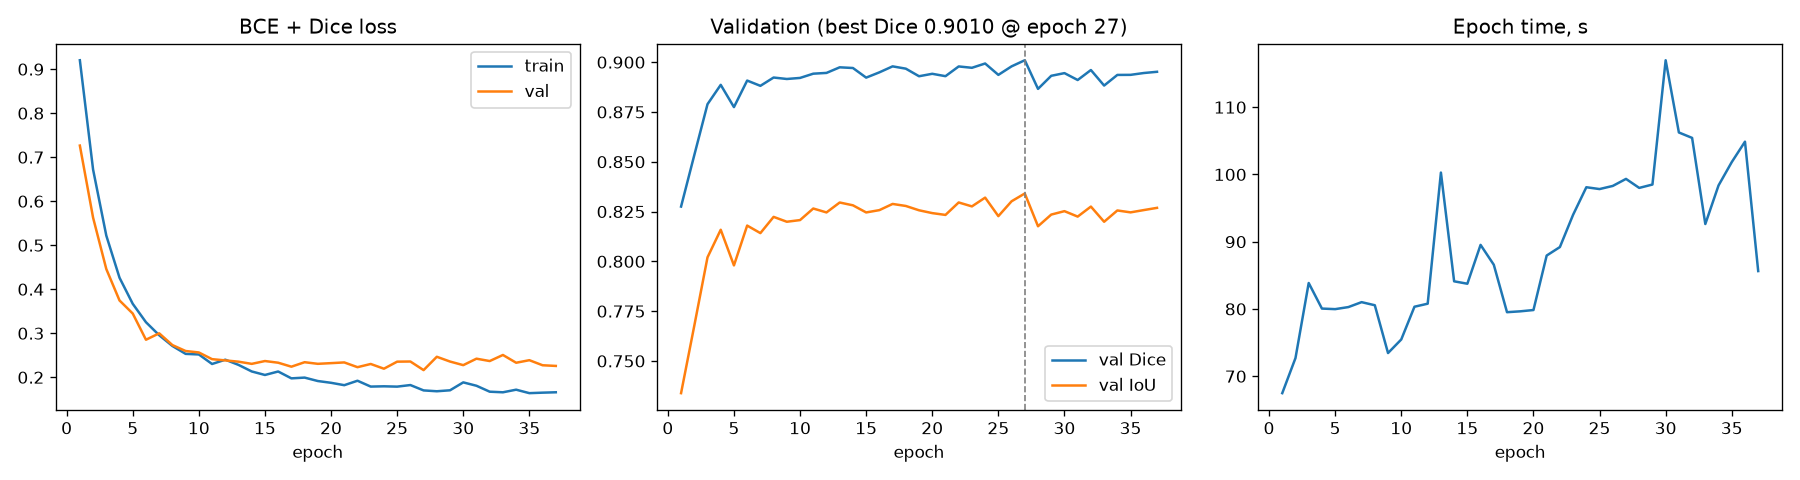
\includegraphics[width=0.9\linewidth]{figures/learning_curves.png}
\caption{Training and validation loss, validation Dice/IoU and epoch time.}
\end{figure}


\section{Observations and Problems}

\begin{itemize}[noitemsep]
  \item \textbf{Training curves:} validation Dice passes 0.89 after 6 epochs and then plateaus at
        0.89--0.90. Training loss keeps decreasing (0.92 $\to$ 0.17) while validation loss
        flattens at about 0.22, so there is mild overfitting after epoch 15.
  \item \textbf{Failure cases:} the worst images are light, low-contrast lesions inside
        immersion-fluid bubbles or contact-plate artefacts, and images with ink markings; the
        model outlines the bubble or a darker neighbouring spot instead of the lesion. These few
        images explain why the mean HD95 (13.7\,px) is almost twice the median (7.2\,px).
  \item \textbf{Harder cases:} seborrheic keratoses and melanomas, which have more irregular and
        less contrasted borders, are segmented worse than nevi; small lesions get a lower Dice,
        although their boundary error in pixels is small (median HD95 3\,px).
  \item \textbf{Annotation noise:} some ground-truth masks are coarse or cover only part of the
        lesion, which limits the achievable Dice.
  \item \textbf{Data leakage:} near-duplicates were not found reliably by pHash; matching all
        image pairs with SIFT was needed (Section~\ref{sec:split}).
  \item \textbf{Implementation bug:} with macOS multiprocessing, every data-loading worker
        received the same copy of the augmentation random generator, so all workers produced
        identical augmentations. We found this in code review before training and fixed it by
        reseeding each worker.
  \item \textbf{Runtime:} the fanless laptop throttles; the epoch time grew from 67\,s to about
        100\,s during training.
\end{itemize}

\section{Next Steps}

\begin{itemize}[noitemsep]
  \item Train DeepLabV3+~\cite{deeplab} with exactly the same split and settings (20 Oct).
  \item Repeat both models with 3 random seeds, as planned, to report mean and standard deviation.
  \item Run the final evaluation of both models on the official 1,000-image test set.
  \item Boundary analysis of the failure cases (low contrast, bubbles and plates, markings).
\end{itemize}

\begin{thebibliography}{9}
\bibitem{isic} N. Codella et al. Skin Lesion Analysis Toward Melanoma Detection 2018: A Challenge
Hosted by the International Skin Imaging Collaboration (ISIC). arXiv:1902.03368, 2019.
\bibitem{unet} O. Ronneberger, P. Fischer, T. Brox. U-Net: Convolutional Networks for Biomedical
Image Segmentation. MICCAI, 2015.
\bibitem{deeplab} L.-C. Chen et al. Encoder-Decoder with Atrous Separable Convolution for Semantic
Image Segmentation. ECCV, 2018.
\end{thebibliography}

\end{document}
